\chapter{SOURCE CODE AND REPRODUCIBILITY}

\section{Repository Structure}

The complete implementation, the executed notebooks, the saved model and the
generated results are kept in a single Git repository. Figure~\ref{fig:arch}
shows how the modules relate: the raw workbook enters through the loader, the
split is written once to \texttt{data/processed/}, and every downstream artefact
is derived from \texttt{results/}.

\begin{figure}[htbp]
\centering
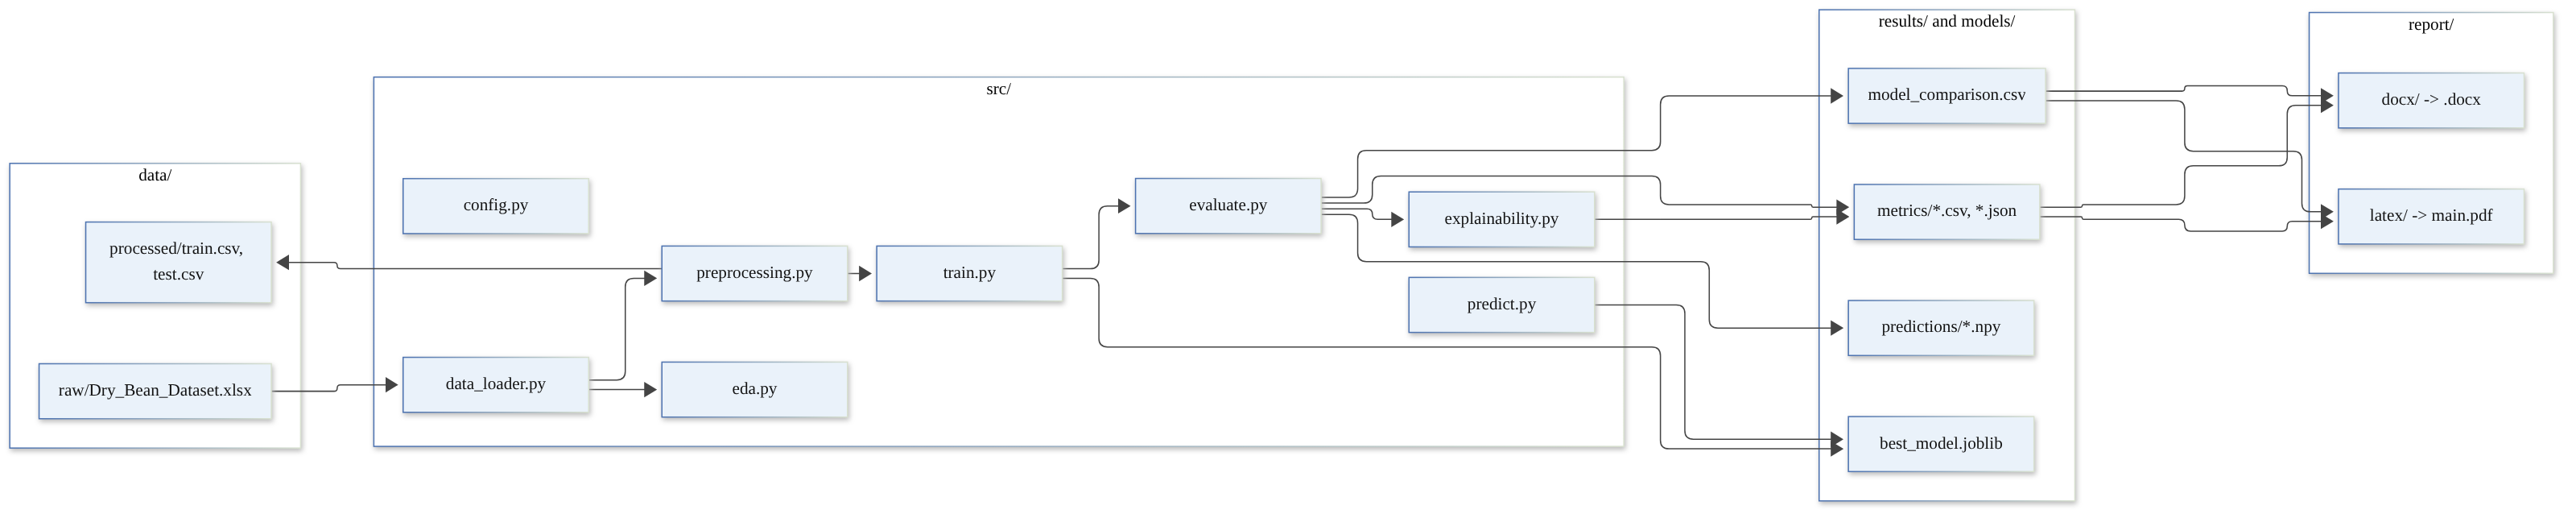
\includegraphics[width=\textwidth]{fig_5_3_architecture.png}
\caption{Module and artefact layout. The report is generated from the files in
\texttt{results/}, not typed from them.}
\label{fig:arch}
\end{figure}

\begin{verbatim}
dry-bean-classification/
├── data/
│   ├── raw/                  Dry_Bean_Dataset.xlsx (downloaded)
│   └── processed/            train.csv, test.csv
├── docs/                     departmental format, mermaid sources
├── figures/
│   ├── eda/                  Chapter 3 and 4 figures
│   ├── models/               Chapter 5 figures
│   └── evaluation/           Chapter 6 figures
├── models/                   six tuned pipelines, best_model.joblib
├── notebooks/                01-04, executed end to end
├── report/
│   ├── latex/                main.tex, chapters/, tables/, references.bib
│   ├── docx/                 Word build of the same content
│   └── final/                compiled PDF
├── results/
│   ├── metrics/              JSON and CSV metric tables
│   ├── predictions/          per-model test predictions
│   ├── model_comparison.csv
│   └── experiment_metadata.json
├── scripts/                  notebook, figure and report builders
├── src/                      pipeline modules
└── tests/                    pytest suite
\end{verbatim}

\section{Installation and Execution}

The pipeline requires Python 3.11 or newer and no GPU. From a clean checkout:

\begin{verbatim}
python3.12 -m venv .venv
source .venv/bin/activate
pip install -r requirements.txt

python -m src.run_pipeline        # download, validate, EDA, train, evaluate
pytest -q                         # 16 tests
jupyter nbconvert --execute --to notebook --inplace notebooks/*.ipynb
python -m src.predict --csv results/predictions/sample_predictions.csv
\end{verbatim}

The dataset is fetched automatically on the first run and cached in
\texttt{data/raw/}. If the machine is offline, placing
\texttt{Dry\_Bean\_Dataset.xlsx} in that directory is sufficient; the loader
skips the download when the file is present.

\section{Determinism}

Four mechanisms make the run reproducible. A single global seed
(\texttt{RANDOM\_STATE = 42}) is used for the split, for every cross-validation
splitter, for every stochastic estimator and for the randomised searches. The
split is written to disk and reloaded by every later stage, so the partition
cannot change between scripts. All searches are deterministic given the seed
because scikit-learn's randomised search draws from a seeded generator. Finally,
the report tables and the number macros in this document are generated from
\texttt{results/} by \texttt{scripts/build\_report\_assets.py}, so a re-run
updates the text rather than leaving stale figures behind.

\section{Key Code}

Listing~\ref{lst:search} shows the search construction. The pipeline, the
scoring rule and the splitter are fixed; only the estimator and its parameter
distribution vary between models.

\begin{lstlisting}[style=pycode, caption={Cross-validated search with the shared
protocol.}, label={lst:search}]
def _search(model_name, spec, split):
    pipe = build_pipeline(spec["estimator"], spec["scale"])
    kwargs = dict(estimator=pipe, scoring="f1_macro",
                  cv=StratifiedKFold(5, shuffle=True, random_state=42),
                  n_jobs=-1, refit=True)
    if spec["search"] == "grid":
        return GridSearchCV(param_grid=spec["params"], **kwargs)
    return RandomizedSearchCV(param_distributions=spec["params"],
                              n_iter=spec["n_iter"], random_state=42, **kwargs)
\end{lstlisting}

Listing~\ref{lst:validate} shows the integrity checks whose output fills
Table~\ref{tab:dataset_summary} and Section~4.1. Nothing is modified at this
stage, so the report can state exactly what was found before any cleaning
decision.

\begin{lstlisting}[style=pycode, caption={Validation reports facts; it never
cleans.}, label={lst:validate}]
def validate(df):
    feature_frame = df[FEATURES]
    corr = feature_frame.corr()
    upper = corr.where(np.triu(np.ones(corr.shape), k=1).astype(bool))
    return {
        "rows": int(df.shape[0]),
        "missing_values_total": int(df.isna().sum().sum()),
        "duplicate_rows": int(df.duplicated().sum()),
        "class_counts_ordered": {k: int((df[TARGET] == k).sum())
                                 for k in CLASS_ORDER},
        "feature_pairs_abs_corr_ge_0.90": {
            f"{a} ~ {b}": float(v)
            for (a, b), v in upper.stack().loc[lambda s: s.abs() >= 0.90].items()},
    }
\end{lstlisting}

\section{Test Suite}

Sixteen tests cover the three failure modes that matter for this project:
corrupted input, leakage, and a broken prediction path. The data tests assert the
verified shape, the absence of missing values, the seven labels and the exact
published class counts. The preprocessing tests assert the split size, that the
stratification holds to within 0.5 percentage points, that the split is
deterministic, that no row appears in both partitions, that the scaler's mean
equals the training mean, and that a standardised kNN is invariant to multiplying
every input by 100. The prediction tests assert that the saved model returns valid
labels, that the reported confidence is the top-3 maximum, that missing and
non-finite inputs are rejected, that the metadata agrees with the comparison table,
and that the command-line entry point returns success.

\chapter{ADDITIONAL RESULTS}

This appendix carries the material that supports the argument of Chapter~6 but is
too detailed for the main text: the fold-by-fold scores behind
Table~\ref{tab:cv_results}, the confusion counts behind
Table~\ref{tab:per_class}, the per-class ROC-AUC behind Figure~\ref{fig:roc}, and
the complete list of strongly correlated feature pairs.

\section{Cross-Validation Stability}

Table~\ref{tab:cv_folds} gives the macro F1 of the selected configuration in each
of the five folds. The spread is what makes the ranking in Table~\ref{tab:cv_results}
fragile: the fold-to-fold range of a single model is comparable to the gap between
adjacent models, so the middle of the leaderboard should not be read as a strict
ordering.

\begin{table}[htbp]
\centering
ootnotesize
\caption{Macro F1 of the selected configuration in each cross-validation fold}
\label{tab:cv_folds}
\begin{tabular}{lrrrrrrr}
\toprule
Model & Fold 1 & Fold 2 & Fold 3 & Fold 4 & Fold 5 & Mean & Std. dev. \\
\midrule
Logistic Regression & 0.9425 & 0.9423 & 0.9321 & 0.9337 & 0.9364 & 0.9374 & 0.0048 \\
K-Nearest Neighbours & 0.9397 & 0.9426 & 0.9324 & 0.9339 & 0.9424 & 0.9382 & 0.0048 \\
RBF-SVM & 0.9491 & 0.9516 & 0.9403 & 0.9391 & 0.9419 & 0.9444 & 0.0056 \\
Random Forest & 0.9364 & 0.9440 & 0.9354 & 0.9366 & 0.9352 & 0.9375 & 0.0037 \\
Extra Trees & 0.9340 & 0.9402 & 0.9332 & 0.9316 & 0.9330 & 0.9344 & 0.0033 \\
Hist Gradient Boosting & 0.9425 & 0.9506 & 0.9379 & 0.9402 & 0.9406 & 0.9424 & 0.0049 \\
\bottomrule
\end{tabular}
\end{table}


\section{Confusion Counts}

Table~\ref{tab:confusion_best} reproduces the counts behind the normalised matrix
in Figure~\ref{fig:cmbest}. Reading it by column rather than by row gives the
precision view: the Sira column receives 50 beans that are not Sira, which is why
its precision is lower than that of the other five large classes.

\begin{table}[htbp]
\centering
\scriptsize
\caption{Confusion matrix of the selected model (RBF-SVM) on the test set}
\label{tab:confusion_best}
\begin{tabular}{lrrrrrrrr}
\toprule
Actual \textbackslash{} Predicted & Seker & Barbunya & Bombay & Cali & Dermason & Horoz & Sira & Recall base \\
\midrule
Seker & 390 & 2 & 0 & 0 & 5 & 0 & 9 & 406 \\
Barbunya & 3 & 242 & 0 & 15 & 0 & 0 & 5 & 265 \\
Bombay & 0 & 0 & 104 & 0 & 0 & 0 & 0 & 104 \\
Cali & 2 & 11 & 0 & 305 & 0 & 6 & 2 & 326 \\
Dermason & 9 & 0 & 0 & 0 & 654 & 0 & 46 & 709 \\
Horoz & 0 & 2 & 0 & 5 & 5 & 367 & 7 & 386 \\
Sira & 8 & 3 & 0 & 0 & 51 & 6 & 459 & 527 \\
\midrule
Total & 412 & 260 & 104 & 325 & 715 & 379 & 528 & 2723 \\
\bottomrule
\end{tabular}
\end{table}


\section{Per-Class Ranking Quality}

Table~\ref{tab:roc_class} reports the one-vs-rest ROC-AUC per variety. Every class
exceeds 0.986, and Bombay reaches 1.000, which separates two different questions:
the model ranks beans of different varieties almost perfectly, but the single
threshold implied by \texttt{predict} still misassigns 7.42\% of them. A
rejection option built on the calibrated probability would exploit that gap.

\begin{table}[htbp]
\centering
\small
\caption{Per-class ROC-AUC of the selected model on the test set}
\label{tab:roc_class}
\begin{tabular}{lr}
\toprule
Variety & One-vs-rest ROC-AUC \\
\midrule
Seker & 0.9982 \\
Barbunya & 0.9959 \\
Bombay & 1.0000 \\
Cali & 0.9964 \\
Dermason & 0.9928 \\
Horoz & 0.9976 \\
Sira & 0.9862 \\
\bottomrule
\end{tabular}
\end{table}


\section{Complete Correlation Structure}

Table~\ref{tab:corr_all} lists all 21 feature pairs with $|r| \ge 0.90$. The
clustering is not random: it follows the algebra of the shape-factor definitions in
Equations~\eqref{eq:roundness}--\eqref{eq:zscore}. Any attribution of importance among the members of a cluster
is therefore arbitrary, as Section~6.7 states.

\begin{table}[htbp]
\centering
ootnotesize
\caption{All 21 feature pairs with $|r| \ge 0.90$}
\label{tab:corr_all}
\begin{tabular}{clr}
\toprule
No. & Feature pair & Pearson r \\
\midrule
1 & Area -- ConvexArea & +0.9999 \\
2 & Compactness -- ShapeFactor3 & +0.9987 \\
3 & Perimeter -- EquivDiameter & +0.9914 \\
4 & AspectRation -- Compactness & -0.9877 \\
5 & ConvexArea -- EquivDiameter & +0.9852 \\
6 & Area -- EquivDiameter & +0.9850 \\
7 & Eccentricity -- ShapeFactor3 & -0.9811 \\
8 & AspectRation -- ShapeFactor3 & -0.9786 \\
9 & Perimeter -- MajorAxisLength & +0.9773 \\
10 & Eccentricity -- Compactness & -0.9703 \\
11 & Perimeter -- ConvexArea & +0.9677 \\
12 & Area -- Perimeter & +0.9667 \\
13 & MajorAxisLength -- EquivDiameter & +0.9617 \\
14 & Area -- MinorAxisLength & +0.9516 \\
15 & MinorAxisLength -- ConvexArea & +0.9513 \\
16 & MinorAxisLength -- EquivDiameter & +0.9485 \\
17 & MinorAxisLength -- ShapeFactor1 & -0.9472 \\
18 & MajorAxisLength -- ConvexArea & +0.9326 \\
19 & Area -- MajorAxisLength & +0.9318 \\
20 & AspectRation -- Eccentricity & +0.9243 \\
21 & Perimeter -- MinorAxisLength & +0.9132 \\
\bottomrule
\end{tabular}
\end{table}

